\documentclass{article}

\author{Pedro Henrique Limeira da Cruz}
\title{ES879 - Sistema de Aquisição de Dados}

\usepackage[margin=0.8in]{geometry}
\usepackage{indentfirst}
\usepackage{fancyhdr}
\usepackage{tcolorbox} 
\usepackage{graphicx}
\usepackage{amsmath}
\usepackage{amssymb}
\usepackage{enumitem}
\usepackage{tabularx} % in the preamble
\usepackage{wrapfig}
\usepackage{subcaption}
\usepackage{multicol}
\usepackage{caption}

% Create a Todo list
\newlist{todolist}{itemize}{2}
\setlist[todolist]{label=$\square$}

\newcolumntype{Y}{>{\centering\arraybackslash}X}
\renewcommand\tabularxcolumn[1]{m{#1}}% for vertical centering text in X column

% Create a new command to be used in the align environment in multiple line equations do only the last equation is numbered  
\newcommand{\n}{\nonumber \\ }
\makeatletter
\let\inserttitle\@title
\makeatother
% Set the style of the page 
\pagestyle{fancy}
\fancyhf{}
\rhead{Pedro Henrique L. da Cruz}
\lhead{\inserttitle}
\rfoot{Page \thepage}

\usepackage{hyperref}
\hypersetup{
    colorlinks=true,
    linkcolor=black,
    filecolor=magenta,
    urlcolor=cyan,
}

% Begin the Document 
\begin{document}

\maketitle
\thispagestyle{empty}

% Add the image inside a figure in as the first page
% \begin{figure}[h]
%     \begin{center}
%         
\includegraphics[scale = 0.15]{/Users/pedrocruz/Documents/UNICAMP/ES101/ES101 - Robotic Arm/img/unicamp.png}
%     \end{center}
% \end{figure}

% Change to the Next page 
\newpage
\tableofcontents
\newpage

\section{Introdução: Sinais, Sistemas e Processamento de Sinais}

\subsection{Definição de Sinal}
Um sinal é definido como qualquer quantidade física que varia com o tempo, espaço, ou outras variáveis independentes. Matemamticamente, nós definimos um sinal por uma função que depende de uma ou várias variáveis, como por exemplo:
\begin{align*}
   s_1(t) &= 5t \\ 
   s_2(t) &= 20t^2
\end{align*}

Onde as funções depende somente de uma variável independente (o tempo), ou ainda como:
\begin{align*}
    s(x,y) = 3x + 2xy + 10y^2
\end{align*}

Que é uma função que depende de duas variáveis ($x, y$) e que, por exemplo, representam as coordenadas em um plano.

Existem, entretanto, sinais onde a sua relação funcional com as variáveis independentes é desconhecida ou ainda muito complicada. Para tais casos, nós somos capazes de representar tais sinais (com um alto nível de fidelidade) através da soma de várias senoides (análogo a uma série Fourier). Um exemplo sendo:
\begin{align*}
    s(t) = \sum^N_{i=1} A_i(t) \sin{[2\pi F_i(t)t + \phi_i(t)]}
\end{align*}

Que pode, por exemplo, representar um eletroencephalograma (EEG), um signal neural ou até mesmo a voz de alguém.

\subsection{Classificação de Sinais}
De forma bem breve, nós podemos classificar um sinal em:
\begin{multicols}{2}
    \begin{itemize}
        \item Sinal Real, $s_1(t) = A\sin(3\pi t)$, ou Sinal Complexo, $s_2(t) = Ae^{j3\pi t}$.
        \item Sinal de 1 canal $s_3(t)$ ou sinal multi-canal $s_4(t) = \{s_a(t), s_b(t), s_c(t)\}$.
        \item Sinal Unidimensional, $s_5(t)$ ou multi-dimensional $s_6(t, x, y)$.
        \item Sinal de tempo contínuo ou discreto (definidos apenas em certos valores de tempo).
        \item Sinal de valor contínuo ou sinal de valor discreto, se um sinal discreto no tempo também assumi valores discretos é chamado de sinal digital.
        \item Sinal determinístico (descrito por uma expressão matemática) ou sinal aleatório.
    \end{itemize}
    \end{multicols}
    
\subsection{Definição de Sistema}
Vimos anteriormente o que seria um sinal. Tais sinais são geralmente gerados a partir da reação a um estimulo por parte de um \textbf{sistema}, sendo que tais estimulos podem ser, por exemplo, uma força, corrente elétrica, luminosidade, etc.
Chamaos também de sistema, qualquer entidade (tanto física quanto digital) que faça operações sobre um sinal. 
Em suma, nós definimos um sistema como:
\begin{itemize}
    \item Uma entidade que gera um sinal a partir de um estimulo.
    \item Uma entidade que faz operações sobre um sinal.
\end{itemize}

Ademais, podemos chamar o conjunto \emph{Estimulo} + \emph{Sinal} de "Signal Source", e a entidade que faz operações em cima do sinal de "sistema de Processamento de Sinais", podendo ser tanto um processamento digital quanto analógico, como iremos ver.
\newpage
\subsection{Elementos Básicos de Sistemas de Processamento de Sinais}
\label{chap:elementos_basicos_processamento_de_sinais}

De forma geral, os sinais que são encontrados na engenharia são, por natureza, analógicos, tendo como variáveis independentes o tempo ou espaço (ambos sendo variáveis contínuas). Tais sinais podem ser processados diretamente no domínio analógicos (e.g por circuitos eletrônicos). 

Na sua forma mais simples, um sistema de processamento analógico de sinais possui uma entrada, uma saída (ambos analógicos), e "processador analógico de sinais", como mostrado na figura abaixo:

\begin{figure}[h!]
    \centering
    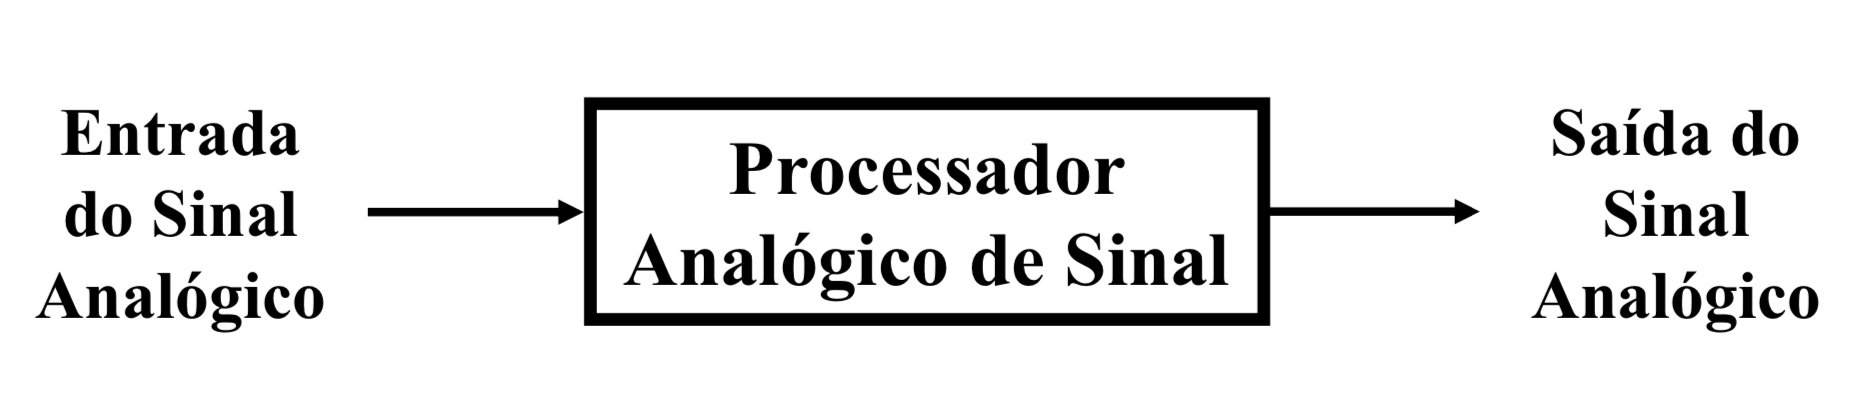
\includegraphics[width=0.5\textwidth]{imgs/filtro_analogico.jpeg}
    \caption{Sistema Básico de Processamento Analógico de Sinais}
    \label{fig:enter-label}
\end{figure}

Existe ainda a possibilidade de fazer o processamento digitalmente (através de micro-processadores/ processadores/ FPGAs), ao invés de analogicamente (por circuitos, etc). Para que possamos fazer isso, entretanto, é preciso que haja um sistema que converta os sinais analógicos e contínuos em sinais digitais que os processadores são capazes de lidar (chamado de \emph{ADC}, ou \emph{Analog To Digital Converter}), e que faça o caminho contrário (converta o sinal processado digitalmente para um sinal analógico), onde usamos um \emph{DAC} (digital do analog converter), resultando no seguinte sistema de processamento:
\begin{figure}[h]
    \centering
    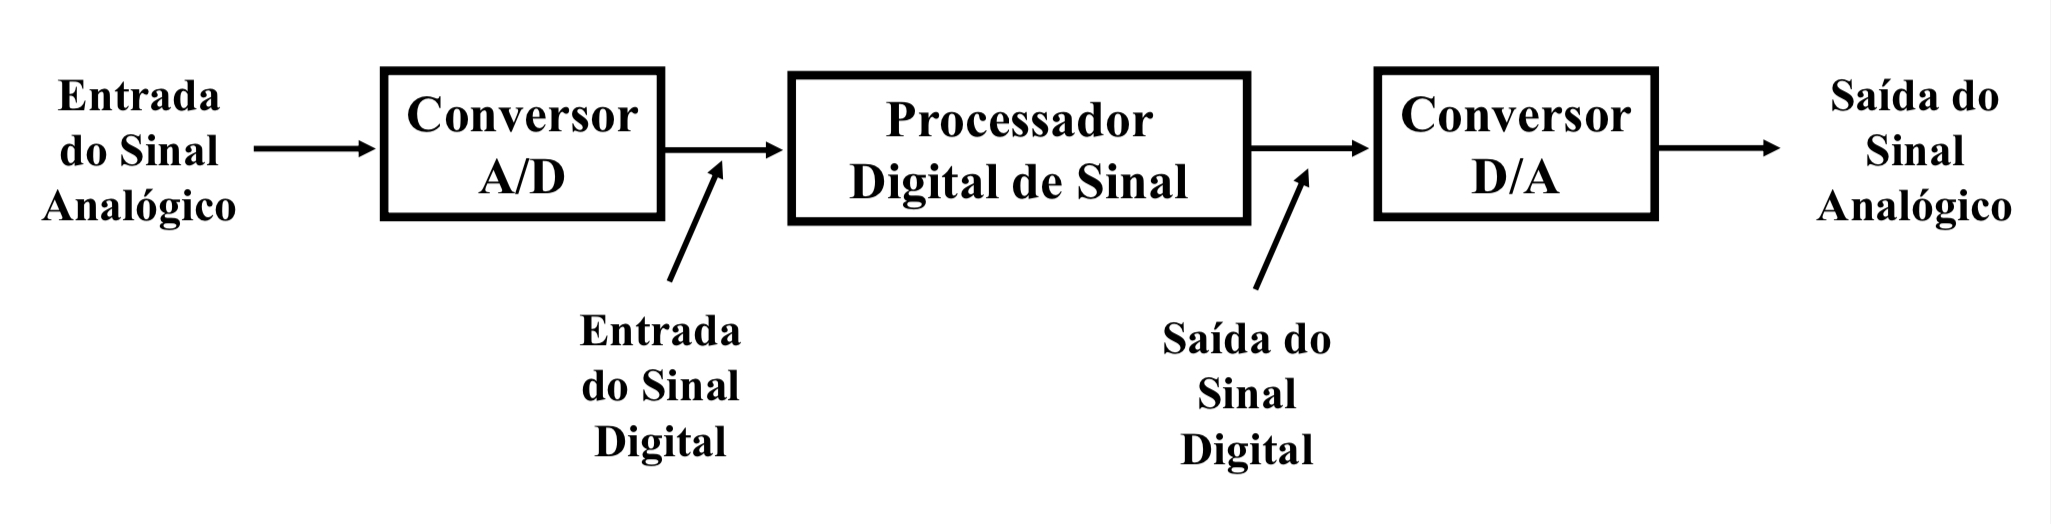
\includegraphics[width=0.7\textwidth]{imgs/filtro_digital.jpeg}
    \caption{Sistema Básico de Processamento Digital de Sinais}
    \label{fig:planta_processamento_digital}
\end{figure}

\subsection{Processamento Analógico V.S Processamento Digital de Sinais}
Vimos anteriormente que o ator que efetivamente faz o processamento do sinal pode faze-lo de forma analógica (sendo implementado fisicamente através de circuitos) ou ainda digitalmente (através de processadores). 

De forma geral, sempre que possível o processamento digital é escolhido por vários fatores, mas os principais sendo:
\begin{itemize}
    \item Maleável - para que uma alteração de implementação seja realizada em um processador digital é muito fácil, basta trocar o programa que estja fazendo o processamento. Já para o processamento analógico, é preciso construir um circuito novo.
    \item Análise dos Dados - analisar os dados digitalmente (através de ferramentas computacionais) é muito mais fácil do que ter que instrumentar o circuito. 
    \item Storage - é muito mais fácil guardar informações na núvem, HD, SSD, entre outros meios que são utilizados no dia a dia do que se tal dado for analógico.
\end{itemize}

Há, entretanto, uma limitação para o processamento digital, sendo ela a diferençca entre frequência do sinal e frequência de amostragem do conversor analógico para digital. Para tais casos, o processamento precisa ser analógico. 

Para ter um entendimento melhor, iremos analizar o conceito de frequência tanto no domínio analógico quanto no domínio digital (ou descreto).
\newpage
\subsection{Conceito de Frequência}
\subsubsection{Frequência no Tempo Contínuo}
Considerando um sinal contínuo no tempo:
\begin{align*}
    x_a(t) = A\cos(\Omega t + \theta)
\end{align*}

Onde tempos que:
\begin{itemize}
    \item $A\rightarrow$ Amplitude
    \item $\Omega\rightarrow$ Frequência, em $[rad/s]$ ou $F = \Omega/2\pi$, com $F = [Hz]$
    \item $\theta\rightarrow$ Fase, em $[rad]$
\end{itemize}

Nós podemos vizualisar algumas propriedades da freqência e de sinais periódicos, sendo elas:

\begin{enumerate}
    \item Para uma frequência $F$ fixa, $x_a(t)$ é periódica $\iff x_a(t+T) = x_a(t)$ para $T=1/f$, chamada de período fundamental.
    \item Se as freuências são diferentes, os sinais são distintos.
    \item Quanto maior a frequência, maior a oscilação.
\end{enumerate}

\subsubsection{Frequência no Tempo Discreto}
\label{chap:freq_discreto}

Analogamente ao sinal contínuo, temos que um sinal de tempo discreto é dado por:
\begin{align*}
    x(n) = A\cos(\underbrace{\omega}_{2\pi f} n + \theta)
\end{align*}

Para que um sinal seja caracterizado como periódico, entretanto, é necessário um rigor a mais quando comparado com sinais de tempo contínuo, tendo que satisfazer as seguintes propriedades, obtidas através da análise de senoides e cossenoides discretas\footnote{Como podemos representar qualquer sinal periódico como uma soma de senos e cosenos, se entendermos as condições de periodicidade de tais relações trigonométricas é possível extrapolar-las para funções periódicas gerais.}:
\begin{enumerate}
    \item $x(n+N) = x(n), \forall n, N>0$, onde $N$ é chamado de \textbf{período fundamental}.
    \item $f \in Q$, i.e a frequência deve ser um número racional (entre dois números inteiros).
    \subitem $\hookrightarrow$ Isso fica claro ao analizarmos um coseno discreto:
    \begin{align*}
        \cos[2\pi f_0 (n+N)] = \cos[2\pi f_0 (n)]
    \end{align*}
    \subitem $\hookrightarrow$ Que é verdade se e somente se $2\pi f_0 N$ (obtido fazendo a distribuitiva dentro do primeiro conseo) for um multiplo de $2\pi$ (valor que representa uma volta no circulo trigonométrico, que representa a volta do $\cos$ ao mesmo valor), podendo ser desconsiderado e então o lado esquerdo da equação será o mesmo do lado direto.
    \subitem $\hookrightarrow$ Matematicamente representamos isso como sendo:
    \begin{align}
        2\pi f_0 N = 2\pi k \Rightarrow f_0 = \frac{k}{N}; \ \ k,N \in \mathcal{Z} \therefore f_0 \in Q
        \label{eq:periodo_fund_disc}
    \end{align}

    \item Sinais discretos cujas frequências são separadas por múltiplos inteiros de $2\pi$ são iguais.
    
    \item Sinais discretos são verdadeiramente distintos se e somente se suas frequências forem $-\pi \leq \omega \leq \pi$ ou $-1/2 \leq f \leq 1/2$. Isso se dá pois a sequência obtida\footnote{Esse é o principal ponto que deve ser compreendido, como estamos lidando com um sinal discreto, no final teremos uma tablea com os dados coletados para cada "instante" $n$, sendo $n$ um inteiro. Pode parecer difícil entender esse conceito principalmente pois pensamos e vizualisamos sempre uma curva contínua, mas se tabelarmos os pontos de tais curvas de alta frequência em intervalos inteiros, veremos que dará um sinal com frequência dentro do intervalo.} de um sinal com frequência fora do intervalo acima será identica a sequência de pontos de um sinal dentro desta faixa, resultando no fenômeno de \emph{aliasing}.
\end{enumerate}

\textbf{EXEMPLO:} Dois sinais discretos distintos apresentam as seguintes frequências fundamentais: $f_1=31/60$ e $f_2 = 30/60$.

Temos que o período fundamental nada mais é do que o menor $N$ tal que o sinal seja periódico. A partir da equação \ref{eq:periodo_fund_disc} temos:
\begin{align*}
    f_1 = \frac{31}{60} = \frac{k}{N} \therefore N = \frac{60}{31}k
\end{align*}

Como temos, por definição, que $N$ e $k$ são inteiros, e $N$ é o menor número inteiro possível, temos que tentar achar o menor valor inteiro de $k$ que gere um valor inteiro de $N$:
\begin{align*}
    N = 60 \iff k = 31
\end{align*}

Já para a segunda frequência temos:
\begin{align*}
    f_2 = \frac{30}{60} = \frac{k}{N} \therefore N = \frac{60}{30}k = 2k
\end{align*}

Logo temos que, o menor número inteiro de $k$ que gere um número inteiro para $N$ é $k = 1 \therefore N = 2$.

\subsection{Amostragem}
\label{chap:amostragem}

\subsubsection{Conceitos Fundamentais}

\begin{wrapfigure}[12]{r}{0.4\textwidth}
\vspace{-20px}
\centering
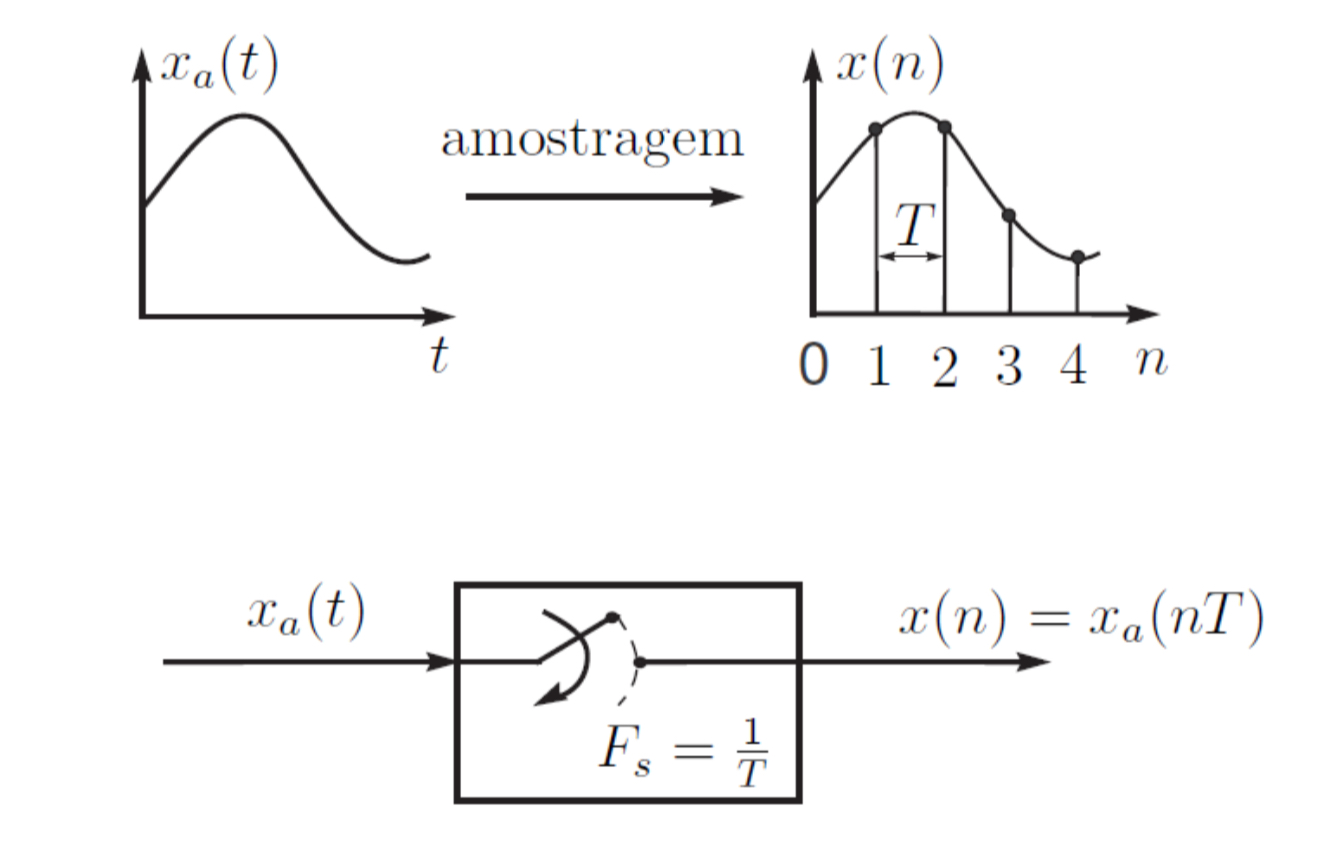
\includegraphics[width=0.4\textwidth]{imgs/ilustration_sampling.jpeg}
\vspace{-15px}
\caption{Modelo de Amostragem}
\label{img:modelo_de_amostragem}
\end{wrapfigure}

Como vimos no capítulo \ref{chap:elementos_basicos_processamento_de_sinais}, onde introduzimos os elementos básicos para processamento de sinais, a primeira etapa para o processamento digital de sinais analógicos é a conversão dos mesmos para o domínio digital, através da amostragem, \emph{i.e} a "captação" desse sinal contínuo em instantes finitos, ou seja, pegamos um sinal contínuo $x_a(t)$ a cada $T$ segundos, ilustrado pela imagem ao lado e representado da seguinte maneira:
\begin{align}
    x(n) = x_a(nT), \ \ \ t=nT=n/F_s
    \label{eq:def_discretizar}
\end{align}

Onde $x(n)$ representa o sinal discretizado\footnote{Para passarmos um sinal da sua forma analógica para discretizada, basta substituirmos $t = n/F_s$ e fazermos as simplificações que derem.} (\emph{i.e} uma sequência de números), e $T$ representa o período de amostragem, resultando na \textbf{frequência de amostragem} $F_s$.

A depender da relação entre a frequencia de amostragem $F_s$ a frequência do sinal contínuo sendo amostrado, pode ocorrer o chamado "aliasing", que, analogamente ao aliasing que ocorrem em sinais discretos com frequência $|F| > 1/2$, um sinal de alta frequência acaba sendo representada por um sinal de frequência baixa, ocorrendo a chamada \textbf{Perda Spectral}.

\subsubsection{Teorema da Amostragem}
A teoria da amostragem determina qual a frequência de amostragem que deve ser usada para \textbf{permitir posteriormente uma adequada reconstrução do sinal}.

Partindo do presusposto de que se sabe a \textbf{frequência máxima} que o sinal de interesse possui $F_{max}$, nós temos que a frequência de sampling \emph{mínima} (também chamada de \textbf{Frequência de Nyquist}):
\begin{align}
    F_N = F_{S_{min}} = 2F_{max}
    \label{eq:nyquist}
\end{align}

Quando o conteúdo de frequência ~e desconhecido, entretanto, estabele-se uma faixa de frequência de interesse e se filtrea o sinal com um filtro analógico passa-baixa (para filtrar todos os sinais fora dessa faixa para evitar contaminação), determinando então o $F_{max}$ antes de fazer a amostragem. Os filtros reais, todavia, não filtram completamente os sinais não desejados (eles são atenuados em uma curva, e não um degrau), por isso é utilizado um fator de segurança, resultando em:
\begin{align}
    F_s > 2F_{max} \times \beta; \ \ \ \beta > 1.5
\end{align}

\newpage
Se a frequêcia de Nyquist (frequÊncia mínima de sampling) não for respeita, pode haver:
\begin{itemize}
    \item Perda nas altas frequÊncias
    \item Ganho nas baixas frequências
    \item Modulação do sinal
\end{itemize}

\textbf{EXEMPLO}: Considerando o sinal analógico $x_a(t) = 5\cos(400\pi t) + \cos(1600\pi t)$, determine a frequência de Nyquist e o discretize.

Para acharmos a Frequência de Amostragem (ou Sampling Frequency), que no caso será a de Nyquist, e sem seguida discretizar o sinal analógico temos que:
\begin{enumerate}
    \item \textbf{Achar Máxima Frequência}: Para tal precisamos escrever todas as frequências dos senos e cossenos explicitamente.
    \begin{align*}
        x_a(t) &= 5\cos(400\pi t) + \cos(1600\pi t) \\ 
               &= 5\cos(2\pi f_1 t) + \cos (2 \pi f_2 t) \\ 
               &= 5\cos(2\pi \cdot 200 \cdot t) + \cos (2 \pi \cdot 800 \cdot t) \therefore \begin{cases}
                   f_1 &= 200 \\ f_2  &= 800 = f_{max}
               \end{cases}
    \end{align*}

    \item \textbf{Calcular $F_N$}: Utilizando a fórmula \ref{eq:nyquist} temos:
        \begin{align*}
            F_s = F_N = 2 \times F_{max} = 2\times F_2 = 1600 Hz
        \end{align*}

    \item \textbf{Discretizar $X_a$}: Para tal, precisamos utilizar a definiçaõ de uma função discretizada, dada pela equação \ref{eq:def_discretizar}, que diz que para discretizar, a partir da frequência de sampling, temos que fazer $t = n/F_s$.
    \begin{align*}
        x(n) &= x_a(n/F_s) \\ 
             &= 5\cos\left(400\pi \frac{n}{1600}\right) + \cos\left(1600\pi \frac{n}{1600}\right) \\
             &= 5\cos\left(n\frac{\pi}{4}\right) + \cos(n\pi) \\
    \end{align*}
\end{enumerate}


\subsubsection{Fenômeno de Aliasing}
Análogo a o que foi descrito no capítulo \ref{chap:freq_discreto}, onde um sinal naturalmente discreto, a depender de sua frequência, pode erroniamente ser descrito por um outro sinal de baixa frequência, um sinal analógico de alta frequência, se amostrado com uma frequência menor que a de Nyquist, também pode acabar sendo representado por um sinal de frequência menor, que chamamos de \textbf{Fenômeno de Aliasing}.

Um exemplo disso é a figura abaixo, onde, ao amostrarmos um sinal de alta frequência a um $F_s$ muito baixo, acabamos identificado um "alias" (ou um ""fantasma"") do sinal real, mas a uma frequência menor:

\begin{figure}[h!]
    \centering
    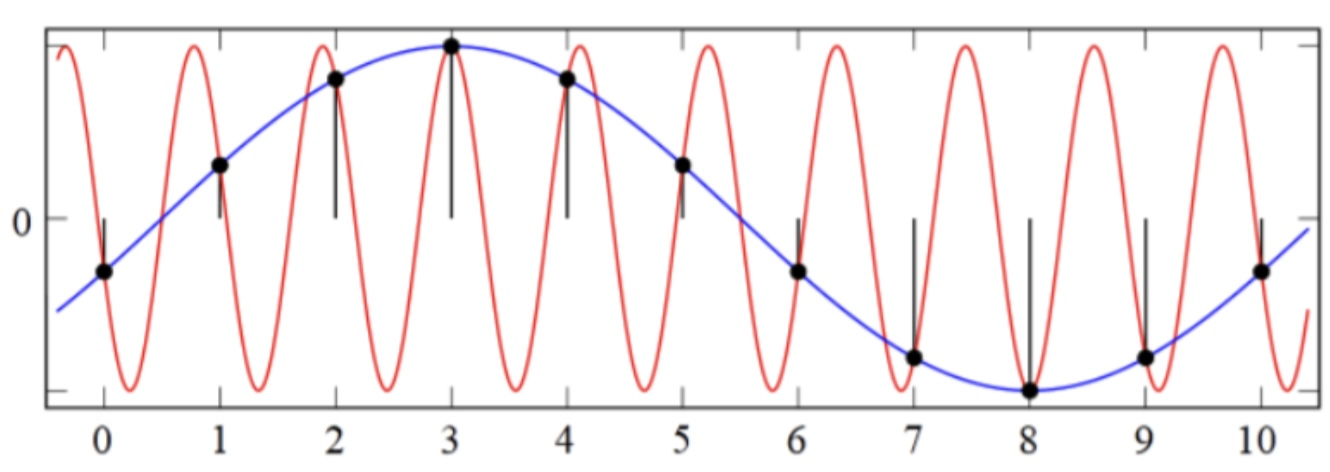
\includegraphics[width=.5\textwidth]{imgs/aliasing.jpeg}
    \caption{Exemplo de Aliasing}
    \label{fig:aliasing}
\end{figure}

\subsubsection{Reconstrução de Sinais}
Quando necessário ,é possível reconstruir o sinal amostrado depois de ter aplicado os processamentos necessários através da conversão $D/A$. Tais conversores interpolam os dados discretos ferando um sinal contínuo, sendo possível as seguintes estratégias de interpolação:
\begin{itemize}
    \item Segurador de Ordem Zero (ZOH) - Segura o valor atual até o príxmo valor.
    \item Segunrador de ORdem Um (FOH) - Faz uma interpolação linear entre os pontos.
    \item Interpolador Cúbico - Realiza uma interpolação cúbica entre os pontos através de \emph{cubic splines}.
\end{itemize}

\subsection{Conversão Analógico-Digital}
Acabmos de ver que é possível, através da teoria de amostragem, transformar um sinal do domínio do contínuo em um sinal discreto. Iremos, agora, ver como é possível pegar esses valores discretos e "digitaliza-los", para que possamos aplicar as diversar estratégias de processamento digital de sinais. Iremos, então, ver primeiro como representamos números em computadores e posteriormente iremos introduzir o conceito de \textbf{Quantização}.

\subsubsection{Números Binários}
Todos os computadores nos quais fazemos o processamento digital de sinais operam em um sistema numérico que chamamos de binário, \emph{i.e} representam seus número na base 2 (através dos digitos $(0,1)$).

Somos capazes de representar números tanto inteiros quanto fracionados na base binária.

\textbf{Números Inteiros}
\begin{align*}
    N = a_{n-1}2^{n-1}+...+a_22^2 + a_12^1 + a_02^0
\end{align*}

Onde:
\begin{itemize}
    \item $a_0 \rightarrow$ Least Significant bit (LSB)
    \item $a_{n-1} \rightarrow$ Most Significant bit (MSB)
\end{itemize}

\textbf{Numero Fracionário}\footnote{Essa  é apenas uma maneira (a mais simples) mas não é utilizada para a representação de números de ponto flutuante na prática, a utilizada é a $IEE754$}
\begin{align*}
    N = a_{n-1}2^{n-1}+...+a_22^2 + a_12^1 + a_02^0\ \cdot \ a_{-1}2^{-1} + a_{-2}2^{-2}+...
\end{align*}

\subsubsection{Quantização}
O processo de converter um sinal de amplitude contínua em um sinal digital expressando cada valor da amostra como um número finitio de dígitos é chamado de \textbf{quantização}.
O processo de quantização, entretanto, não é perfeito, ocorrendo o chamado "erro de quantização" ou ainda "ruído de quantização".

No processo de quantização, dizemos que:
\begin{itemize}
    \item O $MSB$ representa a metade  do fundo de escala ($FS$)
    \item O $LSB$ corresponde à $2^{-n}$ do fundo de escala, também chamado de \textbf{Resolução} ou \textbf{Nível de Quantização} $q$.
\end{itemize}

Além disso, temos que uma plavra de $n$ bits determina $L = 2^n$ \textbf{estados distintos}, ou seja, possui uma resolução de $1/2^n$.

Como estamos lidando com uma converção de algo que tem uma resolução infinita (o sinal contínuo da natureza) para algo que tem uma resolução finita ($Res = 2^{-n}$, como vimos acima) ocorre uma aproximação. Tal aproximação pode ser feita seguindo duas estratégias distintas:
\begin{itemize}
    \item \textbf{Arredondamento}: Ocorre quando arredondamos o número obtido a depender do primeiro digito menos significativo que não conseguimos representar (\emph{e.g} $3.54 \rightarrow 3.5, 3.56 \rightarrow 3.6$). Possui o maior erro de $\pm q/2$.
    \item \textbf{Truncamento}: Ignoramos o primeiro digito menos significativo que não conseguimos representar, independente de seu valor (\emph{e.g} $3.51 \rightarrow 3.5, 3.59 \rightarrow 3.5$). Possui o maior erro de $\pm q$.

    Para determinarmos a quantidade de bits necessária para representarmos um intervalor de valores entre $x_{min}$ e $x_{max}$, com uma resolução de $\Delta$, temos:

    \begin{minipage}{0.35\textwidth}
        \begin{align}
            n = \log_s L
        \end{align}
    \end{minipage}
    \begin{minipage}{0.5\textwidth}
        \begin{align}
            L = \frac{x_{max} - x_{min}}{\Delta} + 1
        \end{align}
    \end{minipage}
\end{itemize}

Onde o $L$ representa a quantidade de \textbf{níveis de quantização} $q$.

\newpage
\section{Filtros Analógicos}
\subsection{Introdução}
Um filtro analoógico pode ser definido como uma \textbf{Rede Seletiva na Frequência}, \emph{i.e} é uma rede que, a depender da frequência do sinal, pode alterar a amplitude e/ou fase do sinal. Dizemos que as frequências que passam pelo filtro sem alteração estão na \textbf{"Banda de Passagem"}, já as frequências que são influenciadas estão na chamada \textbf{"Banda de Atenuação"} ou ainda \textbf{Banda de Corte}. 

Como os nomes das próprias bandas rementem, as componentes do sinal que estão na banda de atenuação tem-se como objetivo eliminar (ou ao menos atenuar) sua presença no sinal resultante ,já as presentes na banda de pssagem tem-se o objetivo de distorcer o menos possível.

De forma geral, no que tange a funcionalidade e a localização das bandas de passagem e de atenuação os filtros são categorizados em:
\begin{table}[h!]
    \centering
    \begin{tabularx}{\textwidth}{|c|X|}\hline
         \textbf{Nome} & \begin{center}
             
         \textbf{Bode Plot: Ideal V.S Real}  \end{center}\\ \hline
         Filtro Passa Baixa &  \begin{center}
          \begin{minipage}{0.3\textwidth}
              \centering
              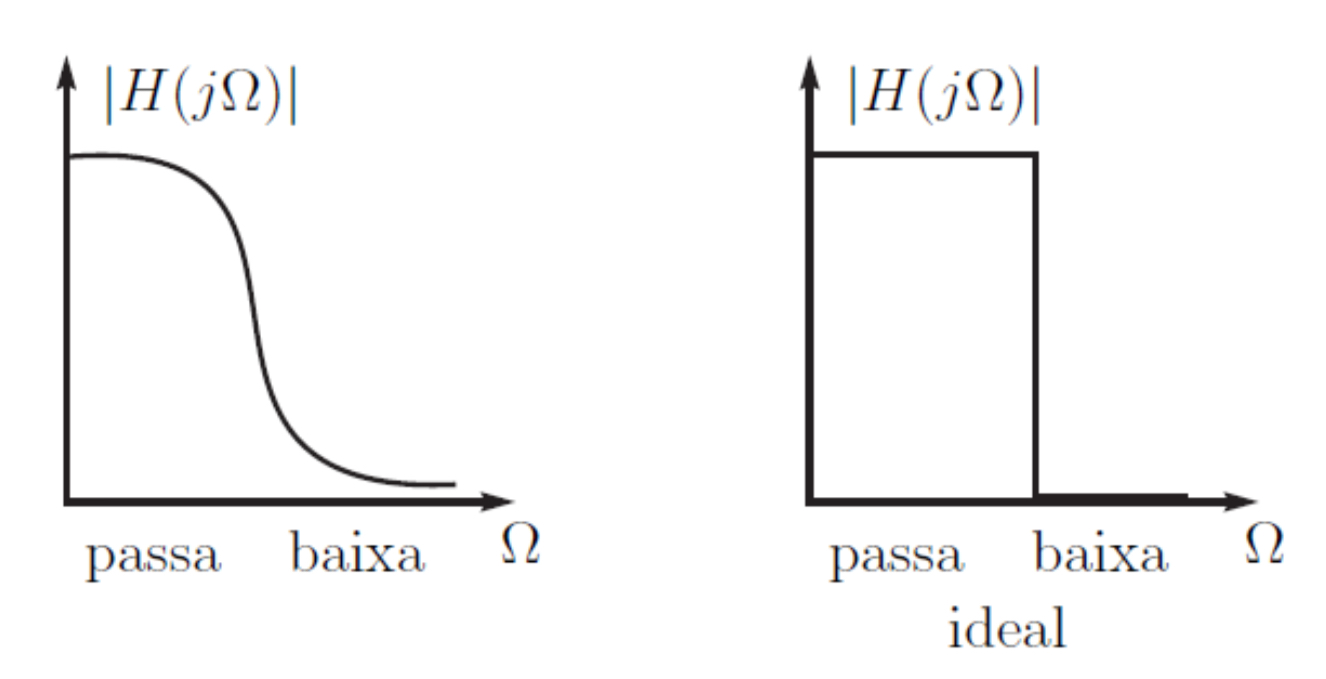
\includegraphics[width=\textwidth]{imgs/passa_baixa.jpeg}
          \end{minipage} \end{center}\\ \hline

          
                Filtro Passa Banda &  \begin{center}
                    
                \begin{minipage}{0.3\textwidth}
              \centering
              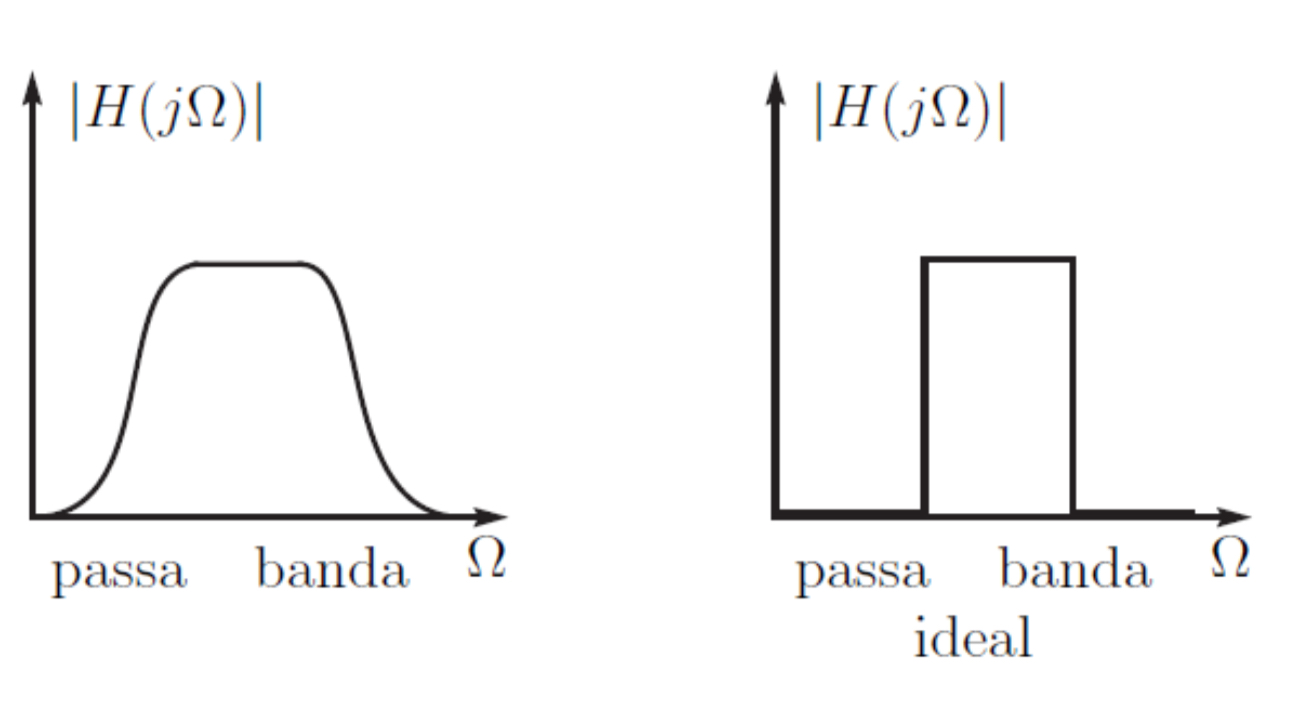
\includegraphics[width=\textwidth]{imgs/passa_banda.jpeg}
          \end{minipage} \end{center}\\ \hline

              Filtro Passa Alta &  \begin{center}
                    
                \begin{minipage}{0.3\textwidth}
              \centering
              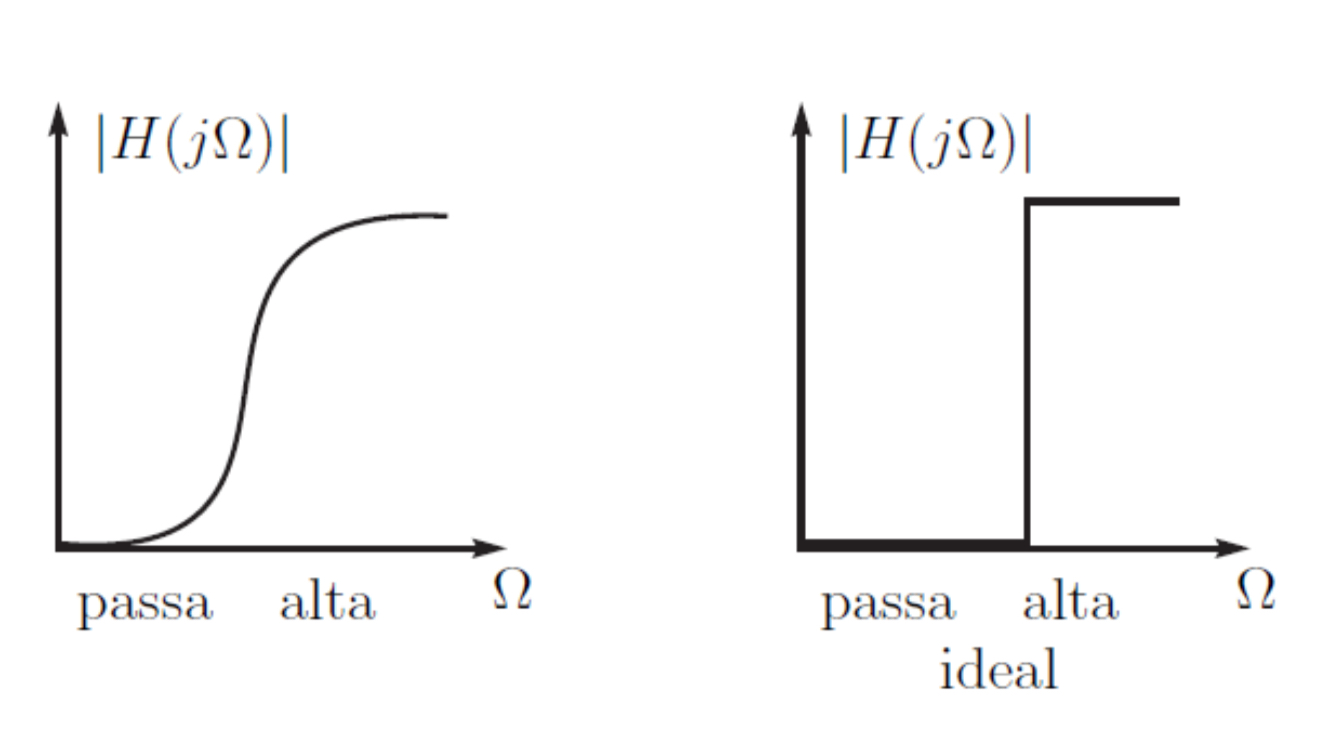
\includegraphics[width=\textwidth]{imgs/passa_alta.jpeg}
          \end{minipage} \end{center}\\ \hline

                          Filtro Rejeita Banda &  \begin{center}
                    
                \begin{minipage}{0.3\textwidth}
              \centering
              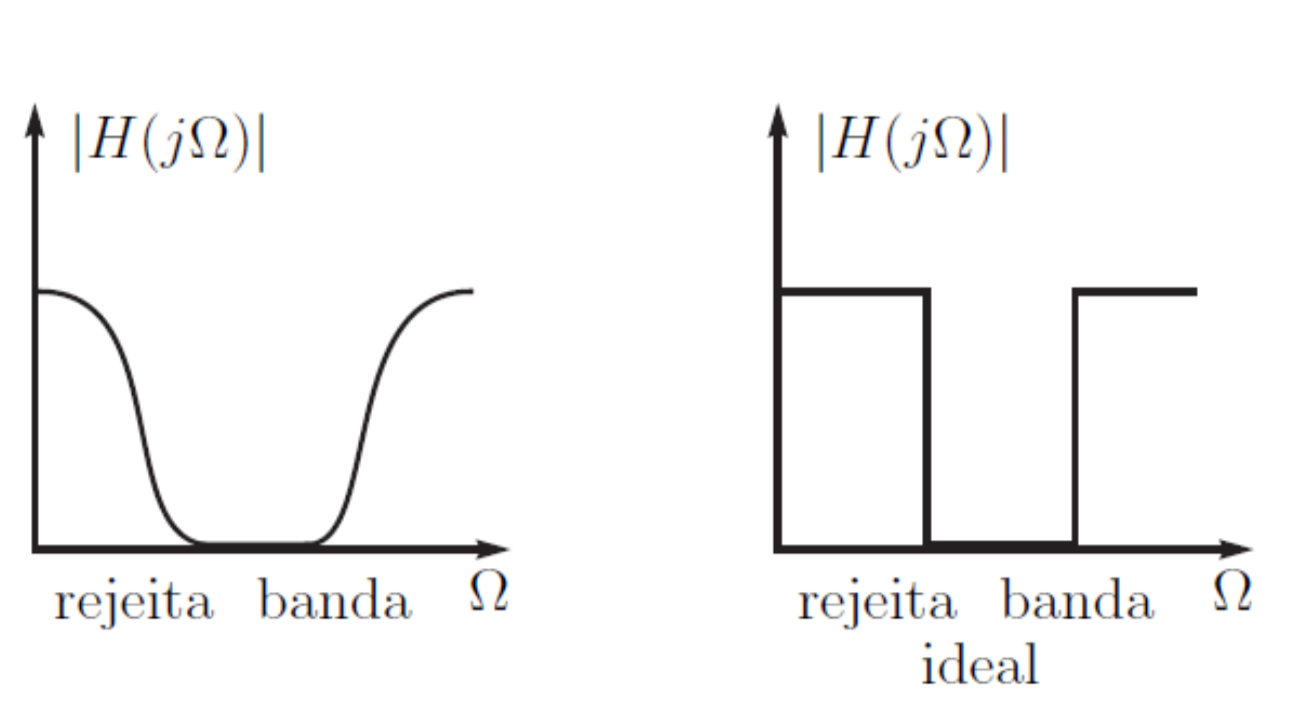
\includegraphics[width=\textwidth]{imgs/rejeita_banda.jpeg}
          \end{minipage} \end{center}\\ \hline
    \end{tabularx}
    \caption{Tipos de Filtros Analógicos}
    \label{tab:my_label}
\end{table}

\newpage
\subsection{Filtros Butter-Worth}

\subsubsection{Função de Transferência}
\begin{wrapfigure}{r}
    \centering
    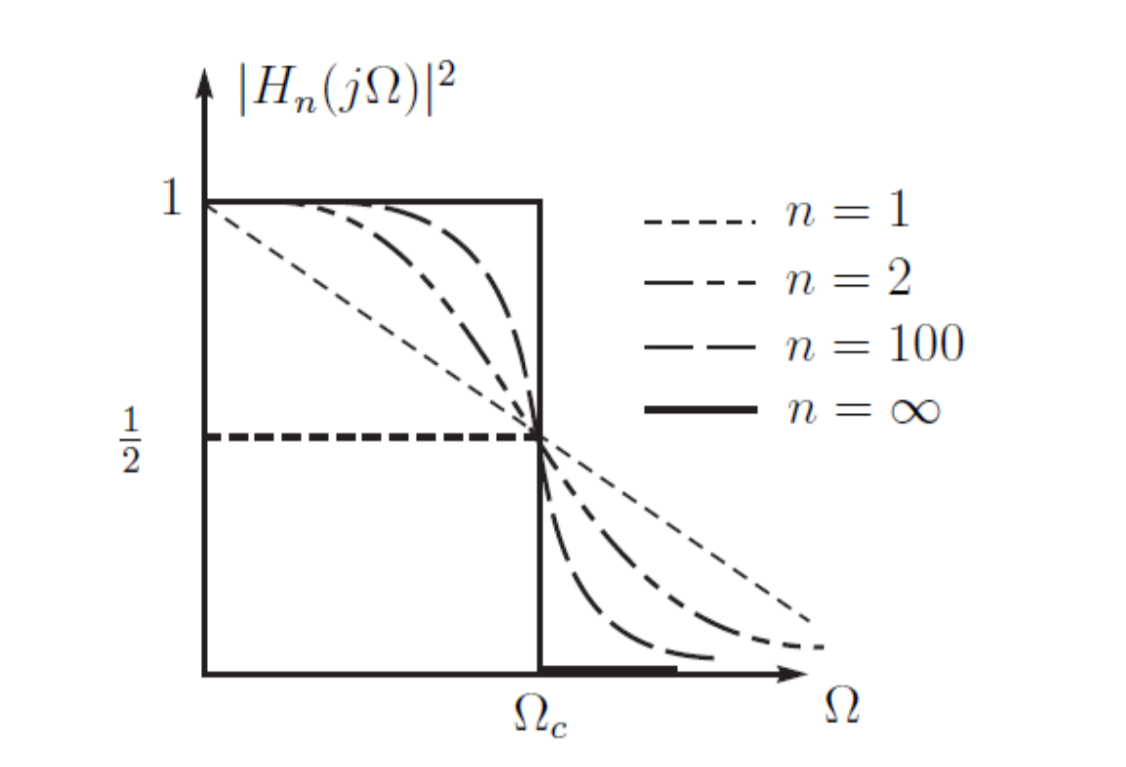
\includegraphics[width=0.4\textwidth]{imgs/butter_worth_tf.jpeg}
    \caption{Butter-Worth Bode Plot}
    \label{fig:enter-label}
\end{wrapfigure}
Um dos principais tipo de filtros analógicos são os chamados de filtros butter-worth. Esse tipo de filtro tem como objetivo chegar o mais perto possível da responsta em frequência (representada pelo bode-plot) teórica, tendo, assim, a resposta o mais reto possível durante a faixa de passagem e uma menor faixa de transição (\emph{i.e} uma menor faixa entre a de passagem e a de corte).

Os filtros Butter-worth são caracterizados pela sua ordem, sendo que, quanto maior a orde (quanto maior o $n$), mais próximo do ideal sua resposta em frequência será (como podemos ver pela imagem ao lado.

Um filtro de ordem $n$, que tem como frequência de corte $\Omega_c$, tem a seguinte função de transferência:
\begin{align}
    |H(j\Omega)|^2 = \frac{1}{1 + \left( \frac{\Omega}{\Omega_c}\right)^{2n}}
    \label{eq:tf_butterworth}
\end{align}

\subsubsection{Estabilidade e Filtro Normalizado}
Vimos anteriormente qual é a função de transferência de um filtro Butter-worth de ordem $n$. Iremos agora, verificar o seu comportamento no que tange sua estabilidade. 

De forma geral, é possível analisar os principais pontos de instabilidade do sistema ao analisarmos a funçaõ de transferência que o representa, e verificarmos os pontos que em seu denominador é zero (ou seja, os pontos em que a resposta do sistema tende a infinito e se torna instavel). Chamaos tais pontos de \textbf{Polos do sistema}.

Para facilitar nossas análises de estabilidade nós iremos:
\begin{enumerate}
    \item \textbf{Utilizar um filtro normalizado $\Omega_c = 1$}. Isso nos possibilitar focar somente na relação entre frequência de entrada $\Omega$ e a resposta do sistema.
    \item \textbf{Analizar a função de Transferência no Plano $s$}. Temos que a função de transferência é obtida ao fazermos a transformada de laplace (a transformada que passa o sistema do domínio do tempo $t$ para o plano $s$ da frequência) da equação diferencial que rege o filtro. A fim de estudarmos a posição dos polos com mais clareza, dentro do plano $s$, iremos fazer a alteração $j\Omega = s \Rightarrow \Omega = s/j$ na equação \ref{eq:tf_butterworth}.

\end{enumerate}

    A partir das considerações acima, podemos ver que a os polos da equação \ref{eq:tf_butterworth} são dados por:
    \begin{align}
        1 + \left(\frac{s}{j}\right)^{2n} = 0 \Rightarrow s^{2n} = -1(j)^{2n}
        \label{eq:polos_butterworth}
    \end{align}

    Considerando que $s = \sigma + j\omega$ (compostos pela soma de uma parte real e uma parte imaginária) temos que a equação acima nada mais é do que a equação de um circulo de raio unitário (tal qual $x^2 + y^2 + \alpha y + \beta x = R^2$) para um plano onde o eixo $x$ é dos números reais e o eixo $y$ é dos imaginários.

    Além disso, considerando que, se a parte real do $s$ for positiva, a transformada inversa de laplace ira resultar em uma exponencial positiva (e por conseguinte tenderá a infinito para $t \rightarrow \infty$), mas caso for negativa ira resultar em uma exponencial com expoente negativo (e por conseguinte ira tender a $0$ para $t\rightarrow \infty$), \textbf{temos que desenvolver um filtro que possua os seus polos, obtidos pela equação \ref{eq:polos_butterworth}, no semi-plano da esquerda (ou seja, possua partes reais negativas).}

    Matematicamente, representamos, então, a fórmula para a funçaõ de transferência como sendo:
    \begin{align}
        H(s) = \frac{1}{\Pi_{SPE} (s - s_k)}
    \end{align}

    Onde $s_k$ representa os polos obtidos na equação \ref{eq:polos_butterworth}, que estão no semi-plano esquerdo.

\section{Análise de Sinais em Frequência}
\subsection{Introdução}
De forma geral, a análise dos sinais no domínio da frequência é uma ferramenta indispensável quando estamos falando de aquisição de dados. Tal análise nos permite, entre outras coisas, identificar todas as diferentes componentes de frequência que um sinal pode ter, sendo elas desejáveis ou não (ruídos). 

A partir da análise das frequências que um sinal possui, somos capazes de projetar o sistema de aquisição mais apropriado, ou ainda desenvolvermos um filtro que tenha como saída somente as bandas de interesse (como vimos na parte de design de filtros analógicos por exemplo).

\subsection{Ferramentas Matemáticas}
As principais ferramentas matemáticas utilizadas para a análise de um sinal no domínio da frequência são:
\begin{itemize}
    \item \textbf{Transformada de Fourier}: Empregada para análise de sinais com energia finita (\emph{i.e} não necessariamente periódicos).
    \item \textbf{Série de Fourier}: Empregada para análise de sinais periódicos.
\end{itemize}

A análise de Fourier de um sinal (que está no dmínio do tempo) faz sua decomposição em componentes senoidais (ou ainda exponenciais complexas, através da identidade de Euler\footnote{A identidade de Euler diz que somos capazes de expressar um sinal senoidal através de exponenciais imaginárias, da seguinte forma: $e^{j\lambda} = \cos{(\lambda)} + j \sin{(\lambda)}$}), gerando o \textbf{Espectro do Sinal}, que pode ser visto como a \emph{assinatura de um sinal no domínio da frequência}.

\subsection{Sinais Contínuos}
\subsubsection{Série de Fourier}

Como dito acima, é possível descrevermos uma senoide tanto pela forma trigonométrica padrão (usando $\sin $ e $\cos$) quanto da forma exponencial complexa. Por causa disso, existem duas formas da série de fourier, sendo ela a exponencial ou trigonométrica, respectivamente.

\begin{minipage}{0.4\textwidth}
    \centering
    \begin{align}
        x(t) &\approx \sum^\infty_{k = -\infty}X_k e^{jk\omega_0 t}, \ \ \omega_0 = 2\pi / T \n
        X_k &= \frac{1}{T}\int^{T/2}_{T/2}x(t) e^{-jk\omega_0t}dt
    \end{align}
\end{minipage}
\begin{minipage}{0.5\textwidth}
    \centering
    \begin{align}
        x(t) &\approx \frac{a_0}{2} + \sum ^\infty _{k=1}[a_k \cos{(k\omega_0t) + b_k \sin{(k\omega_0t)}}] \n
        a_k &= \frac{2}{T}\int^{T/2}_{T/2}x(t) \cos{(k\omega_0t)} dt, \ k = 0, 1, 2, ... \n
        b_k &= \frac{2}{T}\int^{T/2}_{T/2}x(t) \sin{(k\omega_0t)} dt, \ k = 0, 1, 2, ...
    \end{align}
\end{minipage}

Onde temos que o coeficiente\footnote{Os Slides do Thiago e a apostila do Serpa usam $c_k$ para $X_k$, mas acho mais fácil esguir a notação $X_k$, oriunda da apostila do Camino de Análise Linear de Sistemas} $X_k$, da série exponencial de Fourier, e os coeficientes $a_k$ e $b_k$ da série trigonométrica, se relacionam da seguinte forma: 
\begin{align}
    a_k^2 + b_k^2 = 4|X_k|^2
\end{align}

Geralmente, os coeficientes são números complexos, e portanto requerem dois gráficos para sua representação (um da parte real e um para a parte imaginária). A forma mais comum, entretanto, de representarmos os espectros de Fourier do sinal é utilizando um gráfico de módulo (chamado de \textbf{Espectro de Amplitude}) e um de fase (\textbf{Espectro de fase}).

\newpage
\subsubsection{Densidade Espectral Sinais Periódicos}
A partir da densidade espectral, somos capazes de identificar quais frequências tem mais influências no sinal. Matematicamente, temos que a potência é dada por:

\begin{minipage}{.5\textwidth}
    \begin{align}
        P_x &= \sum^\infty_{k = -\infty} |X_k|^2 \\ 
        P_x &= a_0^2 + \frac{1}{2}\sum^\infty_{k = 1} (a_k^2 + b_k^2)^2
    \end{align}

     Onde cada elemento da somatória representa a "influência" da $k$-ésima frequência ($0, 1F_0, 2F_0, ...$) no sinal.
\end{minipage}
\begin{minipage}{0.5\textwidth}
    \centering
    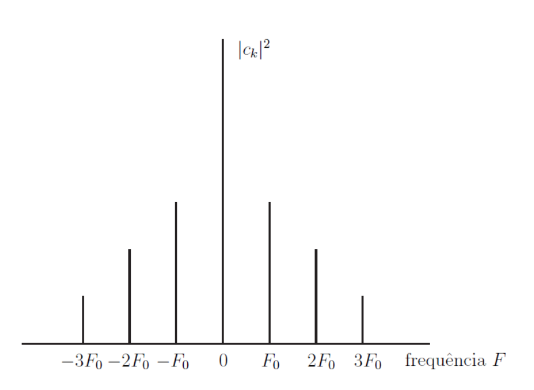
\includegraphics[width=0.8 \textwidth]{imgs/espectro_potencia.png}
\end{minipage}

\subsubsection{Transformada de Fourier}
Analogo a análise que somos capazes de fazer para sinais periódicos, também somos capazes de analisar o espectro de sinais não periódicos.

Tendo como base a série de Fourier, temos que o espectro é formado por linhas igualmente espaçadas, cujo tal espaçamento é a frequência fundamental $F_0$ do sinal. Extrapolando tal ideia, temos que quando a período do sinal cresce, menor fica o espaçamento entre tais linhas e, por conseguinte, quando temos um sinal com período tendendo a infinito $T \rightarrow \infty \therefore f \rightarrow 0 \therefore$ \textbf{não periódico} teremos um espectro contínuo.

Tal \textbf{espectro contínuo, que caracterísa sinais não periódicos}, é obtido através da seguinte definição da \textbf{Transformada de Fourier}:

\begin{align}
    X(\Omega)  = \int ^{+\infty} _{-\infty} x(t) e^{-j\Omega t} dt, \ \ \ \Omega = 2\pi F
\end{align}

\subsubsection{Densidade Espectral de Energia de Sinais  Não-Periódicos}

A paritr da relação de Parseval, temos que a Energia de um sinal é definida como:
\begin{align}
    E_x = \int ^{+\infty}_{-\infty} |x(t)|^2 dt = \int ^{+\infty}_{-\infty} |X(F)|^2 dF = \int ^{+\infty}_{-\infty} S_{xx}(F)dF
    \label{eq:energia_sinais_con_n_periodicos}
\end{align}

Onde o termo $S_{xx}(F) = |X(F)|^2$ representa a distribuição de energia do sinal como uma função da frequência e caracteriza a \textbf{Densidade Espectral de Energia}, \emph{i.e} através da transformada de Fourier somos capazes de achar $X(F)$ e, por conseguinte, determinar a densidade espectral de um sinal, obtendo uma representação de cada frequência do sinal e sua contribuição para o sinal final, como visto na imagem da densidade espectral de sinais periódicos.

Um caso mais específoc, onde um sinal possui somente componentes de frequência entre $F_1 < F < F_1+\Delta F$ podemos simplificar a integral da equação de energia do sinal (eq \ref{eq:energia_sinais_con_n_periodicos}) para:
\begin{align}
    E_x = \int ^{F_1 + \Delta F}_{F_1} S_{xx}(F)dF
    \label{eq:energia_sinais_con_n_periodicos}
\end{align}

\newpage
\subsection{Sinais Discretos}

\subsubsection{Série de Fourier}
Seja um sinal periódico $x(n) = x(n + N)$ de período $N$. A representação da sua série de Fourier é expressa como:
\begin{align}
    x(n) = \sum^{N-1} _{k = 0} X_k e^{j2\pi k n / N}; \ \ \ X_k = \frac{1}{N}\sum^{N-1}_{n = 0} x(n)e^{-j2\pi k n /N}
\end{align}

Onde os coeficientes $X_k$ representam o sinal $x(n)$ no domínio da frequência.

\subsubsection{Densidade Espectral de Potência - Sinais Perioódicos}
Analogamente ao cenário contínuo, para sinais discretos perioódicos temos que sua energia é dada por:
\begin{align}
    E_N = \sum^{N-1}_{n=0} |x(n)|^2 = N\sum^{N-1}_{n=0} |X_k|^2
\end{align}

Onde os valores $|X_k|^2$ representam a \textbf{densidade espectral de potência} do sinal periódico.

\subsubsection{Transformada de Fourier de Tempo Discreto}
Para sinais discretos não periódicos, temos que a transformada de Fourier é dada por:
\begin{align}
    X(\omega) = \mathcal{F}[x(n)] = \sum^\infty _{n=-\infty} x(n) e^{-j\omega n}
\end{align}

Onde $X(\omega)$ representa o conteúdo de frequência de x(n).  Já a transformada inversa é dada por: 
\begin{align}
    x(n) = \mathcal{F}^{-1}[X(\omega)] = \frac{1}{2}\int^\pi _{-\pi}X(\omega)e^{j\omega n}d\omega
\end{align}

Algo importante de ressaltar é que um sinal terá uma transformade de Fourier se e somente se ela seja absolutamente somável\footnote{Nos exercícios é importante lembrar do critério de convergência de séries geométricas, que diz que uma série $\sum ^\infty _{n = 1} a r^{n-1} = \frac{a}{1 - r} \therefore conv. \iff |r| \le 1$}, \emph{i.e}:
\begin{align}
    \exists\mathcal{F}[x(n)]  \iff \sum^{+\infty} _{-\infty} x(n) < \infty
\end{align}
Temos, ainda, que a transformada de fourier possui algumas propriedades que facilitam a sua análise e seu calculo, sendo elas:
\begin{enumerate}
    \item \textbf{Periodicidade:} $X(\omega) = X(\omega + 2\pi)$
    \item \textbf{Simetria:} Se $x(n)$ é um sinal real, então $X(\omega) = X^*(\omega)$. Nesse caso, apenas $\omega \in [0,\pi]$ é suficiente para a análise do sinal.
    \item \textbf{Linearidade:} $\mathcal{F}[\alpha x_1(n) + \beta x_2(n)] = \alpha \mathcal{F}[x_1(n)] + \beta \mathcal{F}[x_2(n)]$
    \item \textbf{Trnaslação no Tempo:} $\mathcal{F}[x(n-k)] = X(\omega) e^{-j\omega k}$
    \item  \textbf{Translação na Frequência}: $\mathcal{F}[x(n) e^{j\omega_0n}] = X(\omega - \omega_0)$
    \item  \textbf{Conjugado}: $\mathcal{F}[x^*(n)] = X^*(-\omega)$
    \item  \textbf{Convolução}: $\mathcal{F}[x_1(n) * x_2(n)] = X_1(\omega) X_2(\omega)$
\end{enumerate}

\subsubsection{Densidade Espectral - Sinais Não Periódicos}
A energia de um sinal $x(n)$ pode ser escirta através da relação de Parseval como:
\begin{align}
    E_x = \sum^\infty _{n=-\infty} |x(n)|^2 = \frac{1}{2\pi} \int^\pi _{-\pi} |X(\omega)|^2 d\omega
\end{align}

A partir do qual definimos $S_xx = |X(\omega)|^2$ como a \textbf{Densidade Espectral de Energia} do sinal $x(n)$ para uma certa frequência $\omega$.

\subsection{Teorema da Amostragemdo Ponto de Vista da Frequência}
O primeiro passo para entendermos abordarmos o teorema de amostragem no ponto de vista da frequência é ter um bom entendendimento de sistemas discretos. 

Os sistemas discretos tem inúmeras similaridades aos sistemas contínuos, por isso alguns conceitos serão desenvolvidos no domínio contínuo e depois somente feito o paralelo para o domínio discreto, tendo em vista nossa maior familiaridade com o primeiro.

\subsubsection{Sistemas Lineares e Shift-Invariant}
No domínio \textbf{contínuo}, o tipo de sistema mais estudado é o chamado \textbf{Sistema Linear e Invariante no Tempo}, o qual possui as seguintes propriedades:
\begin{enumerate}
    \item \textbf{Linearidade:} Se a entrada de um sistema $x_1(t)$ gera uma saída $y_1(t)$, e a entrada $x_2(t)$ gera a saída $y_2(t)$. Se uma entrada $x_3(t) = \alpha x_1(t) + \beta x_2(t)$, composta de uma combinação linear de $x_1$ e $x_2$ for posta no sistema, sua resposta será uma combinação linear das saídas $y_3(t) = \alpha y_1(t) + \beta y_2(t)$
    \item \textbf{Invariância no Tempo:} Para uma entrada $x_1(t)$, a saída do sistema é $y_1(t)$. Se essa mesma entrada for aplicada, mas em um tempo $T$ depois, $x_1(t + T)$ ele resultara em $y_1(t + T)$. Na prática, isso implica que não importa qual instante é o considerado $t = t_0$
\end{enumerate}

Além disso, para sistemas lineares, invariantes no tempo e contínuo temos que \textbf{a equação  $h(t)$ que modela o sistema é a resposta do próprio sistema a uma entrada inpulso $\delta (t)$}. A partir de tal modelo temos que para uma entrada qualquer $x(t)$ a resposta $y(t)$ é dada pela convolução entre a entrada e a equação que rege o sistema $y(t) = x(t) * h(t) = h(t) * x(t)$.

Partindo da convolução como uma forma de acharmos a resposta do sistema a partir de sua resposta ao impulso, temos que, para uma entrada exponencial imaginária $x(t) = e^{j \Omega_0 * t}$, a resposta será:
\begin{align*}
    y(t) = x(t) \ast h(t) = h(t) \ast x(t) &= \int^{+\infty}_{-\infty} h(\tau) e^{j\Omega_0 (t-\tau)} d\tau \\
    &= e^{j\Omega_0 (t)} \underbrace{\int^{+\infty}_{-\infty} h(\tau) e^{-j\Omega_0 \tau d\tau}}_{\mathcal{L}[h(t)]} = x(t) H(\Omega_0)
\end{align*}

Onde podemos observar uma das características mais importantes de sistemas LTI:
\begin{center}
    \textbf{Para um sistema LTI, sua resposta será composta por um fator de amplificação e ângulo de fase em relaçõa a entrada, mas tera a mesma (ou as mesmas) frequências do sinal que o excita.}
\end{center}

\newpage
Para sistemas discretos que iremos tratar, chamados de \textbf{Sistemas Lineares e Shift-Invariant (LSI)}, temos que a propriedades de linearidade é identica ao que foi explorado para sistemas contínuos. Já a propriedade de invariância no tempo se traduz para a a \textbf{"shift-invariance"}, isso é: Para um sistema, o qual produz, a partir de uma entrada $x(n)$, uma saída $y(n)$, para uma entrada $x(n-N)$ será produzida uma saída $y(n-N)$.

Além disso, é importante ressaltar que a propriedade que nos diz que \textbf{a equação $h(n)$ que rege o sistema é obtido através da sua resposta a uma entrada impulso $\delta(n)$} ainda é valida, com o único detalhe que, para sistemas discretos nós temos a somatória de convolução, ao invés da integral.

A parte mais importante para nos aprofundarmos no estudo do espectro de sistemas discretos é entendermos que: \textbf{Um sinal, ao passar por um sistema \emph{LSI}, produzirá uma repsosta que irá possuir as mesmas componentes de frequência, mas podendo haver variações nas suas magnitudes e fase.} Que pode ser obtida pela somatoória de convolução e representado como:
\begin{figure}[h]
    \centering
    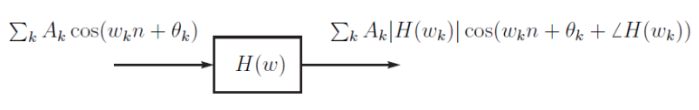
\includegraphics[width=0.7\textwidth]{imgs/tf_discreto.png}
    \caption{Resposta em Frequência - Discreto}
    \label{fig:resposta_em_frequência_discreto}
\end{figure}

Essa informação é importante de termos em mente pois é ela representa que o caminho contrário, partindo da resposta gerada e da planta do sistema e identificarmos o sinal de entrada, é possível.

Fazendo o link com a aplicação em processamento de sinais, é impressindível que seja feita a amostragem correta pois, caso contrário, o sinal discretizado que sera alimentado no sistema de filtro (ou outro algoritmo, mas que possar ser representado por uma função $h(t)$, \emph{i.e} uma função de transferência) terá as componentes de frequência errado e, por conseguinte, irá representar um sinal distorcido.

\subsubsection{Teorema de Amostragem}
Quando falamos do teorema de amostragem, vimos que se não houver uma frequência de sampling alta o bastante, o que ocorre é o alisasing, que é o fenômeno onde as componentes de alta frequência que não foram amostradas corretamente "infectam" as componentes de menor frequência. 

Isso é ainda mais visível quando olhamos os spectros de frequência dos sinais, pois o overlap é ainda mais notável, como podemos ver pela imagem abaixo, onde a figura superior foi amostrada com frequência suficiente, enquanto na debaixo não:
\begin{figure}[h]
    \centering
    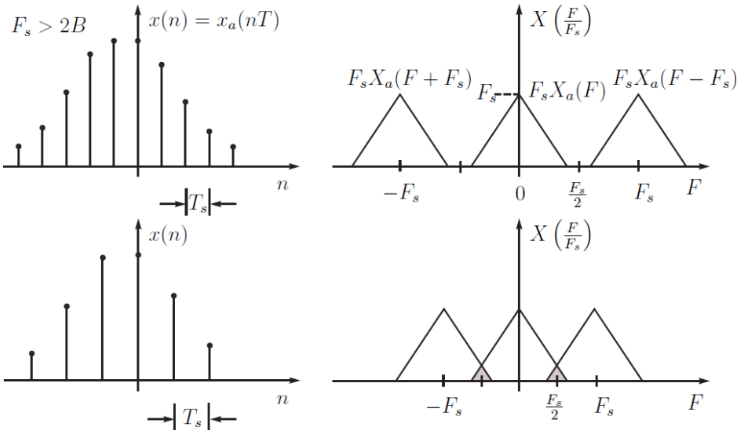
\includegraphics[width=0.5\textwidth]{imgs/aliasing_freq.png}
    \caption{Aliasing no Domínio da Frequência}
\end{figure}

Temos que o aliasing causado por uma frequência $F_a$, que não segue a condição de Nyquist ($F_s = 2F_{max}$), irá contaminar as frequências (chamadas de frequência contaminada $F_{cont.}$), que é calcualda pelas seguintes relações:
\begin{align}
    F_a = \{F_{cont.} + n \cdot F_s \ , \ F_{cont.} - nF_s \ , \ F_s - F_{cont.} \}
\end{align}

Resultando no spectro da frequência contaminâda $F_{cont.}$ sendo acrescida do spectro que seria da frequência $F_a$.

\subsection{Transformada Discreta de Fourier}
\subsubsection{Equacionamento}
Até o momento, vimos que somos capazes de calcular a transformada de Fourier para sinais contínuos e sinais discretos. No que tange sinais discretos, vimos como fazer a transformada a partir de fórmula que descreve o sinal discreto, o que na maioria das vezes não temos. 

Isso ocorre com frequência quando estamos analisando e fazendo o processamento de dados com computadores (ou quase todos os sistemas atuais) que utilizam sinais discretos (ou ainda discretizados), os quais temos apenas os pontos coletados, e não a equação que os gerou, e devido a isso não somos capazes de aplicar a transformada de tempo discreto neles, mas sim a \textbf{Transformada Discreta de Fourier}.

A trasnformada Discreta de Fourier $X[k]$ pode ser pensada como uma amostragem da transformada de tempo discreto $X(\omega)$, sendo descrita como:
\begin{align}
    X[k] = X\left(\omega = \frac{2\pi k}{N}\right) = \sum^{N-1}_{n = 0} x(n) e^{-j\frac{2\pi}{N}kn}
\end{align}

E a transformada inversa sendo:
\begin{align}
    x(n) = \frac{1}{N}\sum^{N-1}_{k = 0} X[k]e^{j \frac{2\pi}{N}nk}
\end{align}

\subsubsection{Propriedades}
A transformada discreta possui as seguintes propriedades:
\begin{itemize}
    \item \textbf{Linearidade}: $ax_1(n) + bx_2(n) \longleftrightarrow aX_1[k] + bX_2[k]$
    \item \textbf{Periodicidade}: $x(n+N) = x(n) \therefore X[k+N] = X[k]$
    \item \textbf{Simetria Circular}: Consideramos que os $N$ pontos $x(n)$ que temos são amostras de um sinal que se repete indefinidamente $x_p(n)$. Logo temos que uma sequência qualquer $x'(n)$ será nada mais que a mesma sequência $x(n)$ defasada por um $k$, que representamos por $x'(n) = x(n - K)_{N}$
    \begin{figure}[h]
        \centering
        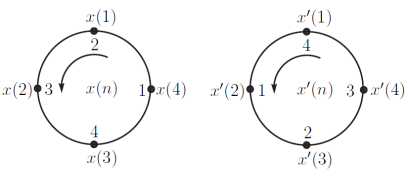
\includegraphics[width=0.5\textwidth]{imgs/circular.png}
    \end{figure}
    \item \textbf{Convolução Circular}: Analogamente a transformada de Laplace e transformada de Fourier de tempo discreto, temos que a convolução (nesse caso convolução circular) ao ser tranformada pela $DFT$ será somente a multiplicação: 
    \begin{align}
        x_1(n)\odot x_2(n) = \sum^{N-1}_{m = 0}x_1(m) x_2((n-m)_{N}) = X_1[k]X_2[k]
    \end{align}
\end{itemize}

\newpage
\section{Filtros Digitais}
Nós iremos abordar 2 tipos distintos de filtros digitais, sendo eles:
\begin{itemize}
    \item \textbf{Filtros FIR:} "Finite Impulse Response" são filtros que, assim como o nome diz, possui uma resposta ao impulso finitas (i.e tendem a zero ao passar do tempo), além de não seremm implementados recursivamente ou com feedback (o que os torna sempre estáveis). A característica mais cobiçada dos filtros, entretanto, FIR é que eles possuem uma respota de fase linear\footnote{Isso ocorre pois sua resposta a impulso (que pode ser interpretada analogamente como sua função de transferência) é simétrica}, o que implica que \emph{não há distorção de fase no sinal filtrado}. Eles, todavia, são computacionalmente mais caros de serem rodados quando os comparamos com os filtros IIR.
    \item \textbf{Filtros IIR:} São filtros de resposta inifinta ao impulso, o que implica que sua estabilidade não é garantida, além de haverem distorções de fase. Sua principal vantagem é que são mais "baratos" computacionalmente falando.
\end{itemize}

\subsection{Filtros FIR - Janelado}
A forma mais usual de projetarmos um filtro FIR é utilizando uma tecnica chamada de "janelamento" de filtros IIR, resultando em um truncamento da resposta impulsiva dos filtros IIR. 

O truncamento é feito através da multiplicação da resposta ao impulso $h_d(n)$ do filtro IIR pela janela $w(n)$, que resulta na respota ao impulso do filtro FIR como sendo:
\begin{align}
    h(n) = h_d(n)w(n) \longrightarrow \mathcal{F}\{h(n)\} = H(\omega) = H_d(\omega) * W(\omega)
\end{align}

Resultando na seguinte resposta ao em frequência, como um exemplo:
\begin{figure}[h]
    \centering
    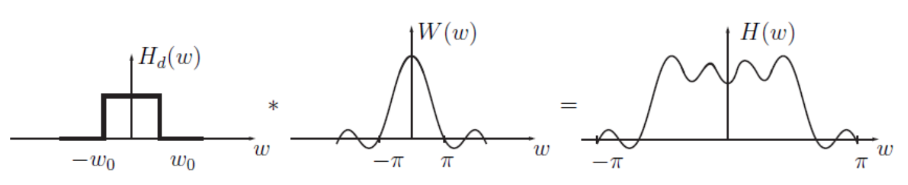
\includegraphics[width=0.8\textwidth]{imgs/filtro_fir_janelado.png}
    \caption{Filtro FIR - Janelado}
\end{figure}

\subsubsection{Principais Janelas}
Existem algumas janelas que são basntante usuais de serem usadas para filtros, sendo elas:

\textbf{Janela Retangular:}
\begin{figure}[h!]
    \centering
    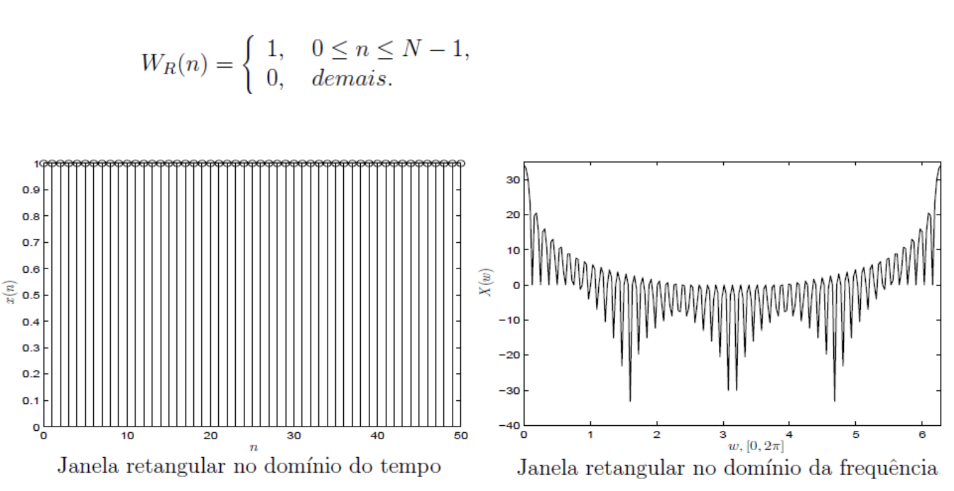
\includegraphics[width=0.7\textwidth]{imgs/janela_ret.png}
\end{figure}

\newpage
\textbf{Janela de Barlett:}
\begin{figure}[h!]
    \centering
    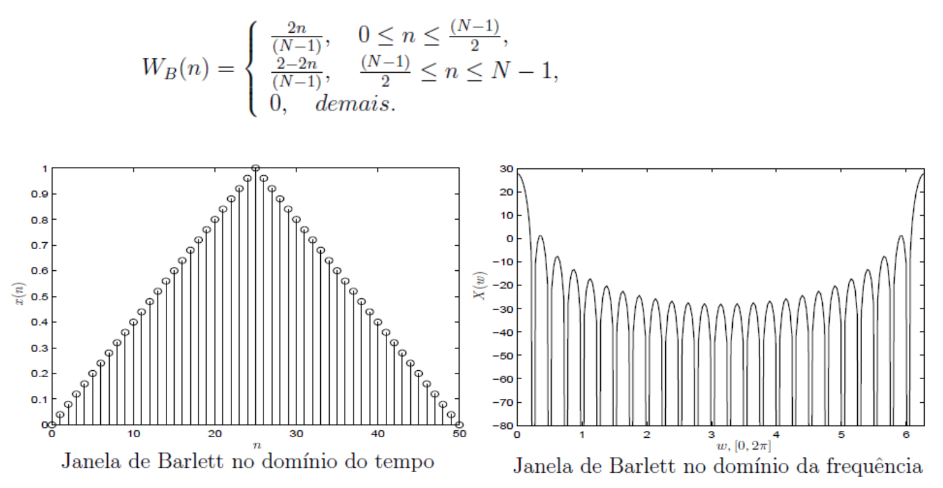
\includegraphics[width=0.7\textwidth]{imgs/janela_barlett.png}
\end{figure}

\textbf{Janela de Hanning:}
\begin{figure}[h!]
    \centering
    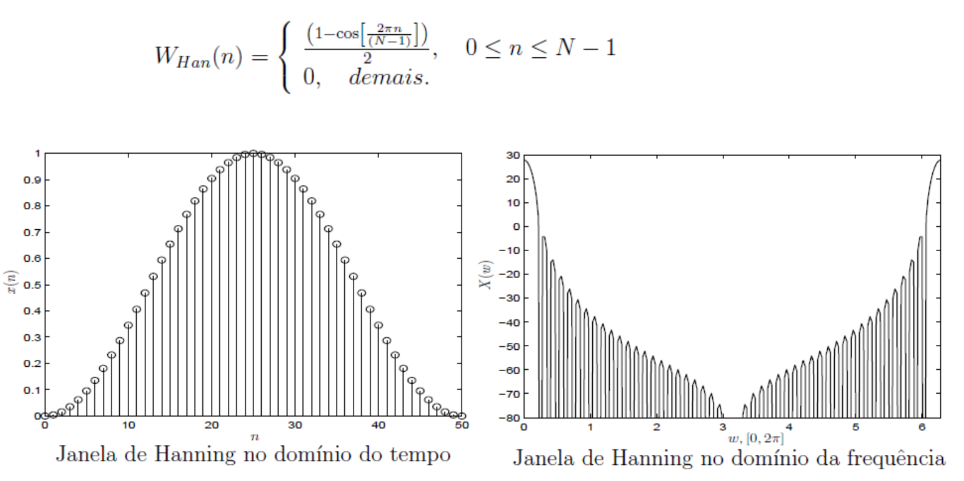
\includegraphics[width=0.75\textwidth]{imgs/janela_hanning.png}
\end{figure}

\textbf{Janela de Hamming:}
\begin{figure}[h!]
    \centering
    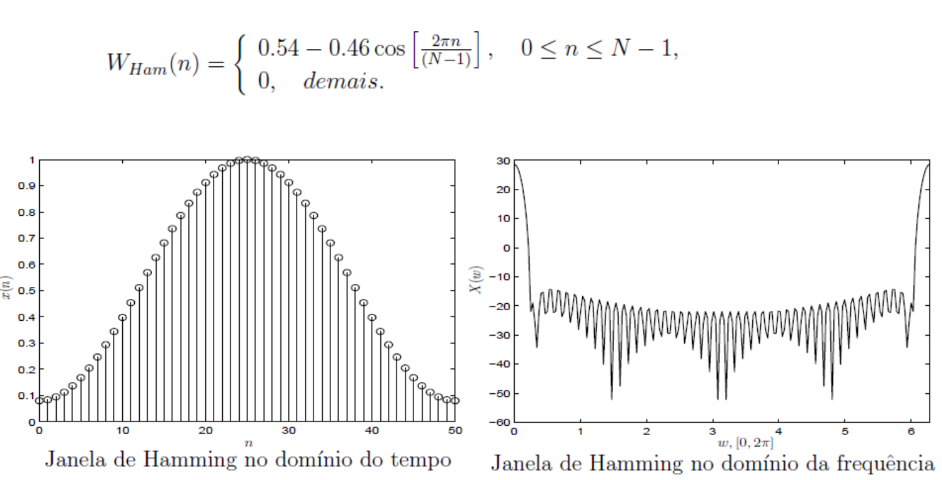
\includegraphics[width=0.75\textwidth]{imgs/janela_hamming.png}
\end{figure}

\newpage
\textbf{Janela de Balckman:}
\begin{figure}[h!]
    \centering
    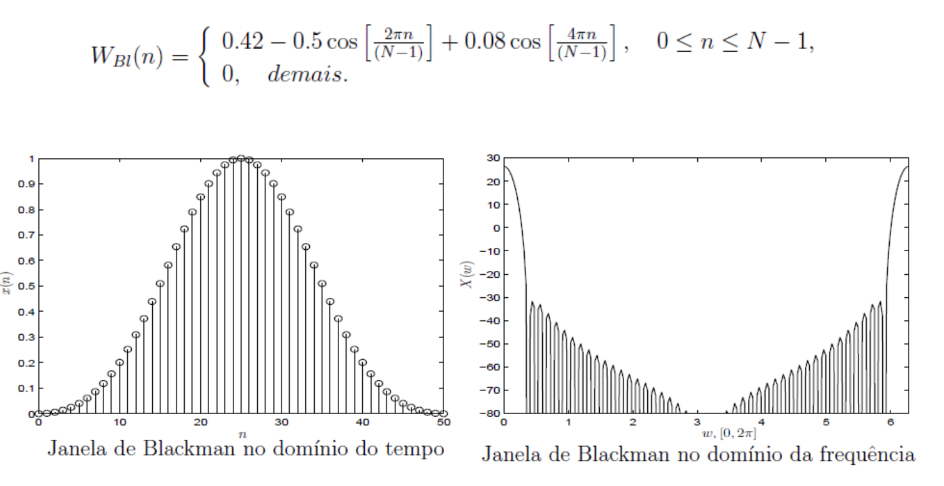
\includegraphics[width=0.75\textwidth]{imgs/janela_blackman.png}
\end{figure}

\subsubsection{Procedimento de Projeto}



\end{document}